




\section{Section 1: Power system of RTS}


In this section is started the literature review of this document, with the coverage of the Railway Transportation System (RTS). This system is reported to transport <<need data>> of people and <<data>> goods. With high influence in the transportation of goods and people in the last century, this system had substantial technological enhancements. Currently we have a RTS with substantial differences in the supply system.

In subsection \ref{subs:311} is presented an overview on European railway electrical supply systems. Later on, in subsection \ref{subs:312}, a comparison between different catenary supply systems is presented and in subsection \ref{subs:313} is presented a comparison of the power system architecture of trains. A further detail on train electrical components is presented in subsection \ref{subs:314}.

This section is supported on the chapter 5 of the work of \cite{abad2016}. Further reading of this book chapter is advisable. 

\subsection{Overview of Existing European Railway Power Systems}
\label{subs:311}
Back to the 19th century, the steam turbine was the main propulsion system for the trains. Later on, electric and diesel propulsion systems were adopted. In recent years occurred a massive introduction of IGBT-based power converters, which allowed an increase of energy efficiency (allowing, for example, regenerative breaking and reduction of power losses in traction motors).

Due to this evolution, different topologies of the railway system exists nowadays. In table \ref{tab:31.t1}, different catenary topologies are visible which results in different power systems for RTS.


% Table generated by Excel2LaTeX from sheet 'Sheet1'
\begin{table}[htbp]
	\centering
	\tiny
	\caption{Catenary topology and vehicle characteristics of different railway vehicles. \cite{abad2016}.}
	\begin{tabular}{|c|p{10.145em}p{10.355em}|cc|}
		\cmidrule{2-5}    \multicolumn{1}{c|}{} & \multicolumn{2}{c|}{\textbf{Catenary topology}} & \multicolumn{2}{c|}{\textbf{Vehicle characteristics}} \\
		\cmidrule{2-5}    \multicolumn{1}{c|}{} & \multicolumn{1}{c}{\textbf{DC supply}} & \multicolumn{1}{c|}{\textbf{AC supply}} & \textbf{Power} & \textbf{Top speed} \\
		\midrule
		\textbf{Tram} & 600V DC, 750V DC, 900V DC & \multicolumn{1}{c|}{-}     & 150–300kW & 50–70km/h \\
		\midrule
		\textbf{Metro} & 750V DC, 1500V DC & \multicolumn{1}{c|}{-}     & 350kW–1MW & 80km/h \\
		\midrule
		\textbf{Train} & 750V DC, 1500V DC, 3000V DC & 15kV AC (16.7Hz) and 25kV AC (50Hz) & 200kW–8MW & 120–350km/h \\
		\midrule
		\textbf{Locomotive} & 750V DC, 1500V DC, 3000V DC & 15kV AC (16.7Hz) and 25kV AC (50Hz) & 500kW–8MW & 100–200km/h \\
		\bottomrule
	\end{tabular}%
	\label{tab:31.t1}%
\end{table}%


Across the Europe, RTS depends on different types of electrification systems, as it is illustrated in figure \ref{fig:abad2016}.


\begin{figure}[h!]
	\centering
	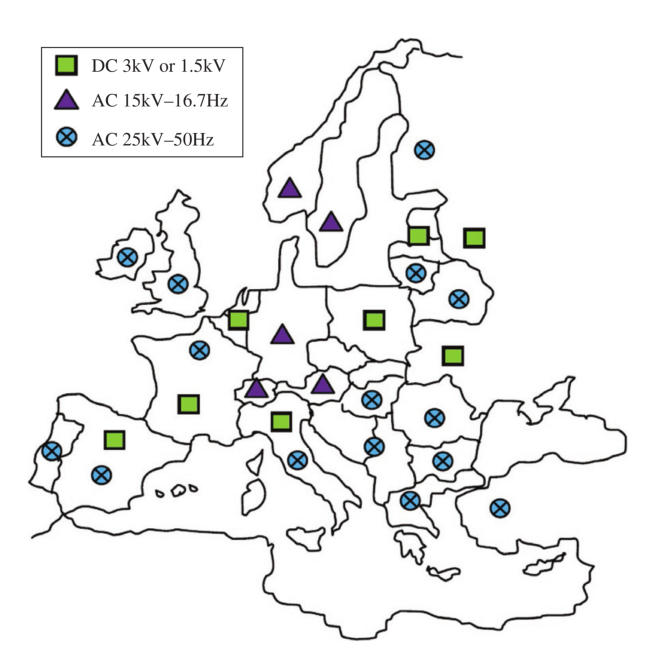
\includegraphics[width=0.7\textwidth,keepaspectratio]{figures/31.PowerS/abad2016}
	\caption{Railway main-line power supply systems in Europe. Adapted from \cite{abad2016}.}
	\label{fig:abad2016}
\end{figure}



\subsection{Railway Power Supply System}
\label{subs:312}

Similarly to the electrical grid where a broad area of loads must be supplied, the railway power system must be capable of maintaining trains running in a broad area. The energy is supplied to the railway system through traction substations, similarly to the generation units of the electrical grid.

These traction substations ensure the interface between the electrical grid and the railway system, being responsible of supplying the distribution line of the railway system - or catenary.

As previously referred, the catenary can be divided in three main topologies:

%\begin{itemize}
%	\setlength\itemsep{-0.5em}
%	
%	\item DC supply system (six-, or 12-pulse diode rectifiers);
%	
%	\item AC 50Hz (or 60Hz) supply system;
%	
%	\item AC 16.7Hz supply system;
%
%\end{itemize}

\paragraph{1. DC supply system\\}

The DC supply system depends on rectifier converters (controlled or uncontrolled) as illustrated in figure \ref{fig:abad2016b}. This railway power supply topology requires several traction substations, towards the reduction of power losses in catenary due to the high value of current. In figure \ref{fig:abad2016f} is presented the supply architecture of such lines.


\begin{figure}[h!]
	\centering
	\begin{minipage}{.5\textwidth}
		\centering
		%		\vspace{2.5em}
		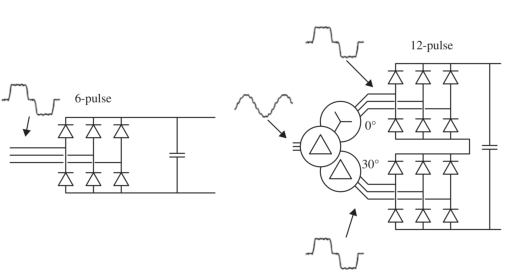
\includegraphics[width=\textwidth,keepaspectratio]{figures/31.PowerS/abad2016b}
		%		\vspace{2em}
		\captionof{figure}{6-pulse and 12-pulse diode rectifier configurations. Adapted from \cite{abad2016}.}
		\label{fig:abad2016b}
	\end{minipage}%
	\begin{minipage}{.03\textwidth}  ~\end{minipage}	
	\begin{minipage}{.4\textwidth}
		\centering
		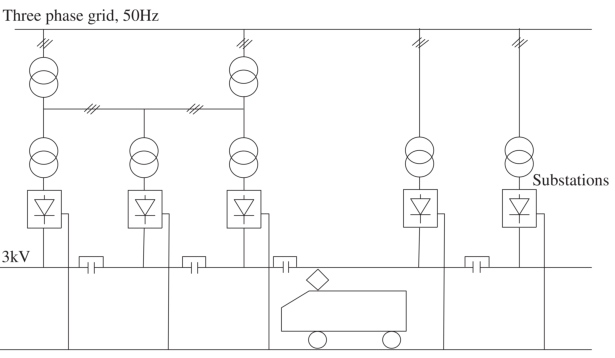
\includegraphics[width=\textwidth,keepaspectratio]{figures/31.PowerS/abad2016f}
		%		\vspace{0.5em}
		\captionof{figure}{DC supply system architecture. Adapted from \cite{abad2016}.}
		\label{fig:abad2016f}
	\end{minipage}
\end{figure}

\paragraph{2. AC 50Hz (or 60Hz) supply system\\}

With AC catenaries, low frequency single-phase transformer is required to step down the catenary voltage (25 kV or 15 kV) to the rectifier operating voltage (the rectifier is a single-phase voltage source converter, usually with bi-directional power flow).

On the traction substation, a special setup of power transformers avoids the usage of complete power converters. In figure \ref{fig:abad2016d} is presented the substation setup to supply a single-phase 50Hz catenary.

\paragraph{3. AC 16.7Hz supply systems\\}
An alternative setup is presented in figure \ref{fig:abad2016e} where a single-phase 16.7Hz supply voltage is generated with a complete power converter. 
%\vspace{-2.5em}


\begin{figure}[h!]
	\centering
	\begin{minipage}{.45\textwidth}
		\centering
		%		\vspace{2.5em}
		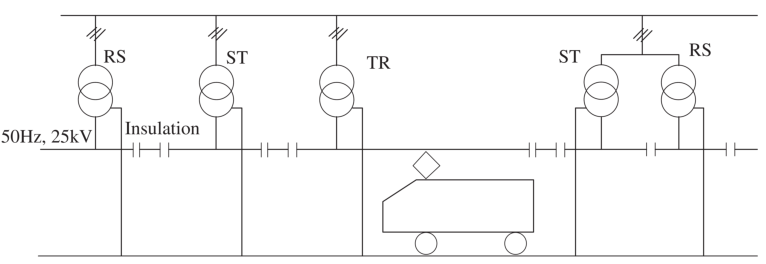
\includegraphics[width=\textwidth,keepaspectratio]{figures/31.PowerS/abad2016d}
		%		\vspace{2em}
		\captionof{figure}{6-pulse and 12-pulse diode rectifier configurations. Adapted from \cite{abad2016}.}
		\label{fig:abad2016d}
	\end{minipage}%
	\begin{minipage}{.03\textwidth}  ~\end{minipage}	
	\begin{minipage}{.45\textwidth}
		\centering
		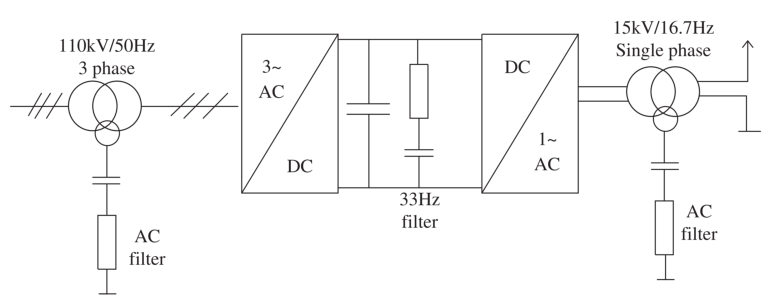
\includegraphics[width=\textwidth,keepaspectratio]{figures/31.PowerS/abad2016e}
		%		\vspace{0.5em}
		\captionof{figure}{DC supply system architecture. Adapted from \cite{abad2016}.}
		\label{fig:abad2016e}
	\end{minipage}
\end{figure}



\subsection{Train Power Supply System}
\label{subs:313}
In this subsection, three types of powering in trains are presented. The first two require a catenary to supply the train and the third are dependent on on-board energy generation (using diesel internal combustion engine).


\paragraph{1. DC supply system\\}


The DC catenary allows an almost direct connection between train power traction and inverter DC bus, as represented in figure \ref{fig:abad2016c}.

\begin{figure}[h!]
	\centering
	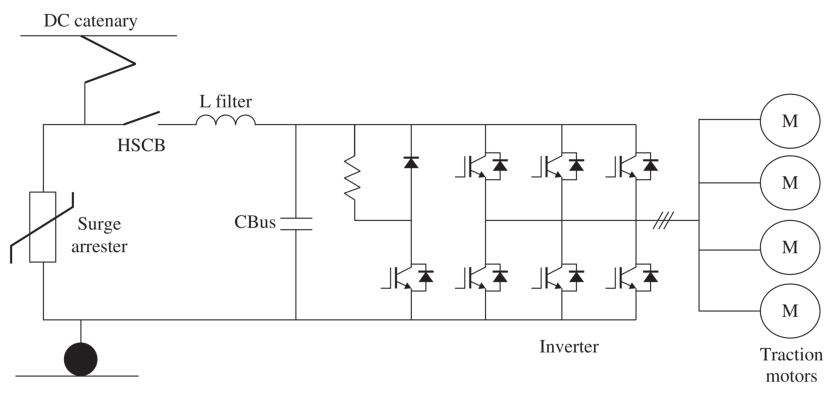
\includegraphics[width=0.65\textwidth,keepaspectratio]{figures/31.PowerS/abad2016c}
	\caption{Train internal power circuit of a DC supply system. Adapted from \cite{abad2016}.}
	\label{fig:abad2016c}
\end{figure}

\paragraph{2. AC supply system\\}

As previously presented, the catenary voltages can be either AC or DC. On the AC catenaries, a single phase transformer and an rectifier is needed to create a DC bus for traction power converters, as presented in figure \ref{fig:abad2016g}.


\begin{figure}[h!]
	\centering
	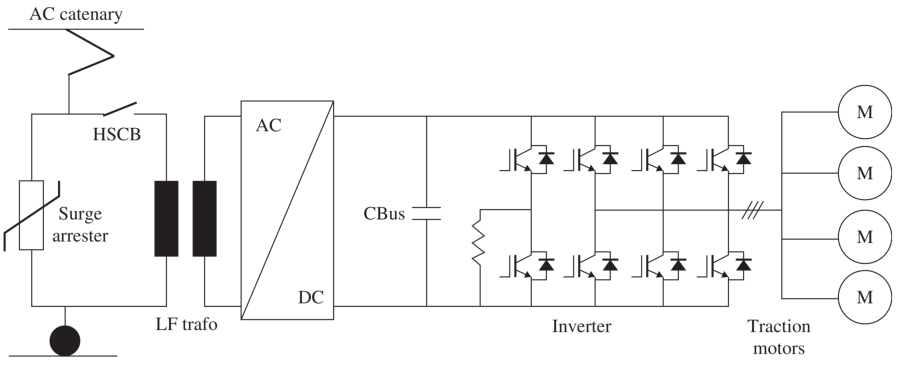
\includegraphics[width=0.65\textwidth,keepaspectratio]{figures/31.PowerS/abad2016g}
	\caption{Train internal power circuit of a AC supply system. Adapted from \cite{abad2016}.}
	\label{fig:abad2016g}
\end{figure}

\paragraph{3. Diesel-electric supply system\\}

An important market share in railway traction is occupied by diesel trains. This type of traction allows the avoidance of catenaries as the power source. The internal power circuit of those trains is presented in figure \ref{fig:abad2016h}.

\begin{figure}[h!]
	\centering
	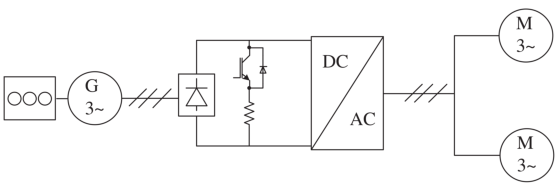
\includegraphics[width=0.55\textwidth,keepaspectratio]{figures/31.PowerS/abad2016h}
	\caption{Train internal power circuit of a Diesel electric locomotive with alternator. Adapted from \cite{abad2016}.}
	\label{fig:abad2016h}
\end{figure}


\subsection{Train Power Components}
\label{subs:314}
\paragraph{1.Pantograph\\}

	The pantograph is a device capable of maintain an electrical contact between train and catenary while in motion.
	
\paragraph{2.Surge Arrester\\}

	This equipment ensures over-voltage protection of train internal circuit, against external events (such as lightings) or internal events (switching faults)
	
\paragraph{3.High-speed Circuit Breaker\\}
	
	This device allows the safe interruption of high current faults.
	
\paragraph{4.Input LC filter\\}

	The main objective is to improve the power quality of the energy supply with the reduction of harmonic distortion (with the absorption of high frequency harmonics and injection of low frequency ones).

\paragraph{5.Filter inductor and DC-link capacitor\\}

	Coupled with electronic power converters/inverters, the filter inductor and DC-link capacitor allows the rectification of the AC voltage into DC. (?)
	
\paragraph{6.Power semiconductors\\}


\paragraph{7.Braking resistor\\}

	Avoid the occurrence of dangerous DC-link voltages (if the main AC grid does not support the generated energy)

\paragraph{8.Power converter box\\}

	Includes the power semiconductors (in power inverter arrangement) and cooling media.

\paragraph{9.Electric traction motor\\}

	Enables mechanical propulsion. The most common technology is the squirrel cage induction motor.


